\documentclass{article}
\usepackage[margin=1in]{geometry}
\usepackage{graphics}
\usepackage{../common}
\usepackage{../pagesetup}

\begin{document}

\lecture{7}{September 25}{Sasha Rush}{Juntao Wang, Alexander Wei, Kevin Zhang, Aron Szanto}{Neural Networks}

\subsubsection{Introduction}

Neural networks have been a hot topic recently in machine learning. But everything we will cover today has essentially been known since '70s and '80s. Since then, there has been in increased focus on this subject due to its successes after improved computing power, larger datasets, better neural network architectures, and more careful study in academia. Neural networks have also seen wide adoption in industry in recent years. Lately, there has also been work trying to integrate other methods of inference into neural networks---we will take a look at this topic later in this course.  We cover neural networks now as a tangentially-related introduction to graphical models and as an example of combining traditional inference with deep models.

\subsubsection{Review of General Linear Models}

In the last lecture, we saw that we can learn a mapping between mean parameters and natural parameters for many general linear models and use squashing functions to change natural parameters into mean parameters.  In general, we describe these models using a transformation $\mu = g^{-1}(w^\top x+b)$ for some function $g$ and a distribution $y \mid x$.

\begin{example}[Linear Regression]
    Here we have $g(x) = x$ (the identity function) with $y \mid x \sim \mathcal{N}(w^\top x+b, \sigma^2)$.  This is the classic model we have already seen.
\end{example}

\begin{example}[Linear Classification]
    In this case, $g^{-1}$ is the sigmoid function $\sigma$, so that $\mu = \sigma(w^\top x+b)$ with $y \mid x \sim\on{Bern}(\sigma(w^\top x+b))$.  We can think of the sigmoid function as a smooth approximation to an indicator variable, so that $\sigma(w^\top x+b)$ is simply an estimation of the class of $w^\top x+b$.
\end{example}

\begin{example}[Softmax Classification]
    Here $g^{-1}$ is the softmax function, so that $\mu_c = \text{softmax}(Wx+b)_c$ where $W$ is some matrix rather than a vector.  Remember that the softmax is defined by $\text{softmax}(z)_c = \frac{\exp(z_c)}{\sum_{c'} \exp(z_{c'})}$.  Think of the softmax function as a sigmoid approximation to multi-dimension.
\end{example}

\subsection{Basis Functions}

It can be advantageous to apply models after modifying the data set using a transformation called a \emph{basis}.  We can have a huge variety of basis functions (some of which we have seen on the problem set), e.g., $\phi_j(x) = \sin(x), \tanh(x), \on{ReLU}(x)$, and so on. Vector examples (i.e., functions on vectors) include $\phi_j(x) = \max\{x_1, x_2\}$ and $\phi_j(x) = x_1 x_2 + x_1^2$. Figuring out a good basis within which to represent data is an important problem in machine learning.

\begin{example}
\label{speech1}

  (Basis Function in Speech Recognition) A snippet of speech might be a waveform, and one way to extract features is to chunk the waveform by time, for each chunk applying a Fourier transform. Then we would take as features some values of each transformed chunk in the frequency domain.  Typically this process gives 13 features per chunk.  These features are then passed to a learning model.
    \begin{figure}[!ht]
    \centering
    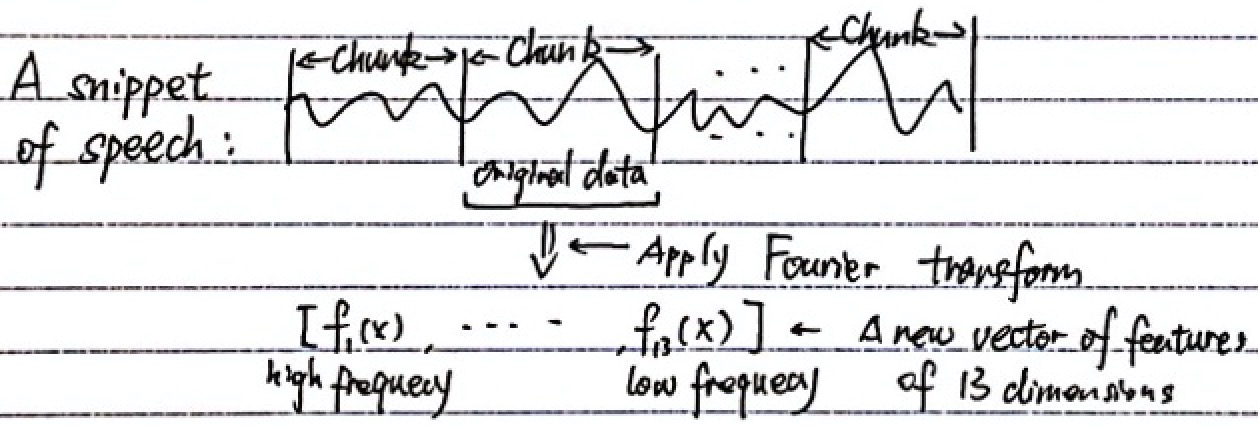
\includegraphics[width = 0.6\textwidth]{speech1.jpg}
    %\vspace{-0.2cm}
    \caption{Fourier transform in speech recognition in Example~\ref{speech1}}
    %\vspace{-0.5cm}
    \end{figure}
\end{example}

We now consider general linear models in combination with basis functions. Suppose $y | x\sim\mathcal{N}(w^\top\phi(x) + b, \sigma^2)$, and $y | x\sim\on{Bern}(\sigma(w^\top \phi(x)) + b)$, where $\phi$ gives rise to a basis. We can do MLE just as before, i.e., compute $\on{argmax}_w \sum_n \log p(y_n | x_n, w)$. In general, these will be solvable just as before, e.g., with numerical optimization---iterative gradient calculation and updates. The form of the MLE depends on the distribution of $y \mid x$. When it is normal, the optimization becomes over sum of squares, when it is Bernoulli, the optimization becomes over cross-entropy (as discussed in previous classes).

\subsection{Now Let's Talk About Neural Networks}

An adaptive basis function is a model with parameters in the basis functions. Neural networks are specific adaptive basis functions with particular structures, which we will describe below.

One can think of the function of a neural net as learning the correct basis function(s) for the data---having the computer come up with the best representation of the data over features of the form $\phi(x; w, b) = g^{-1}(Wx + b)$, where $g^{-1} = \on{relu}, \sigma, \on{softmax}$, or another nonlinear function. This procedure can be applied recursively, e.g., we can define the $x$ that lives inside this basis function to also have its own basis function, e.g., $\phi(x; w, b) = g^{-1}(w\phi'(x; w', b') + b)$, and so on. This is also why neural networks are often referred to as ``deep learning.'' This allows us to do non-linear regression and classification with parameters. Now, when we do regression and classification, we can have complex models such as
$$y | x \sim \mathcal{N}(w^\top\tanh(w'x + b') + b, \sigma^2)$$
When we do MLE, we have to take the same argmax over the parameters $w, w', b', b$. All that's changing is that the function we are optimizing is non-linear, with many parameters, and non-convex. So when we optimize such functions, we might end up at a local optimum instead of the global optimum. We will see many techniques for combating the complexities of non-convex optimization.

\subsection{Demo}

See iPython notebook for demo.

\subsection{Graphical Representation}

Consider the adaptive basis $\sigma(w^\top \sigma(Wx + b') + b)$. We can represent this graphically with a two-layer, fully-connected network:

\begin{center}
    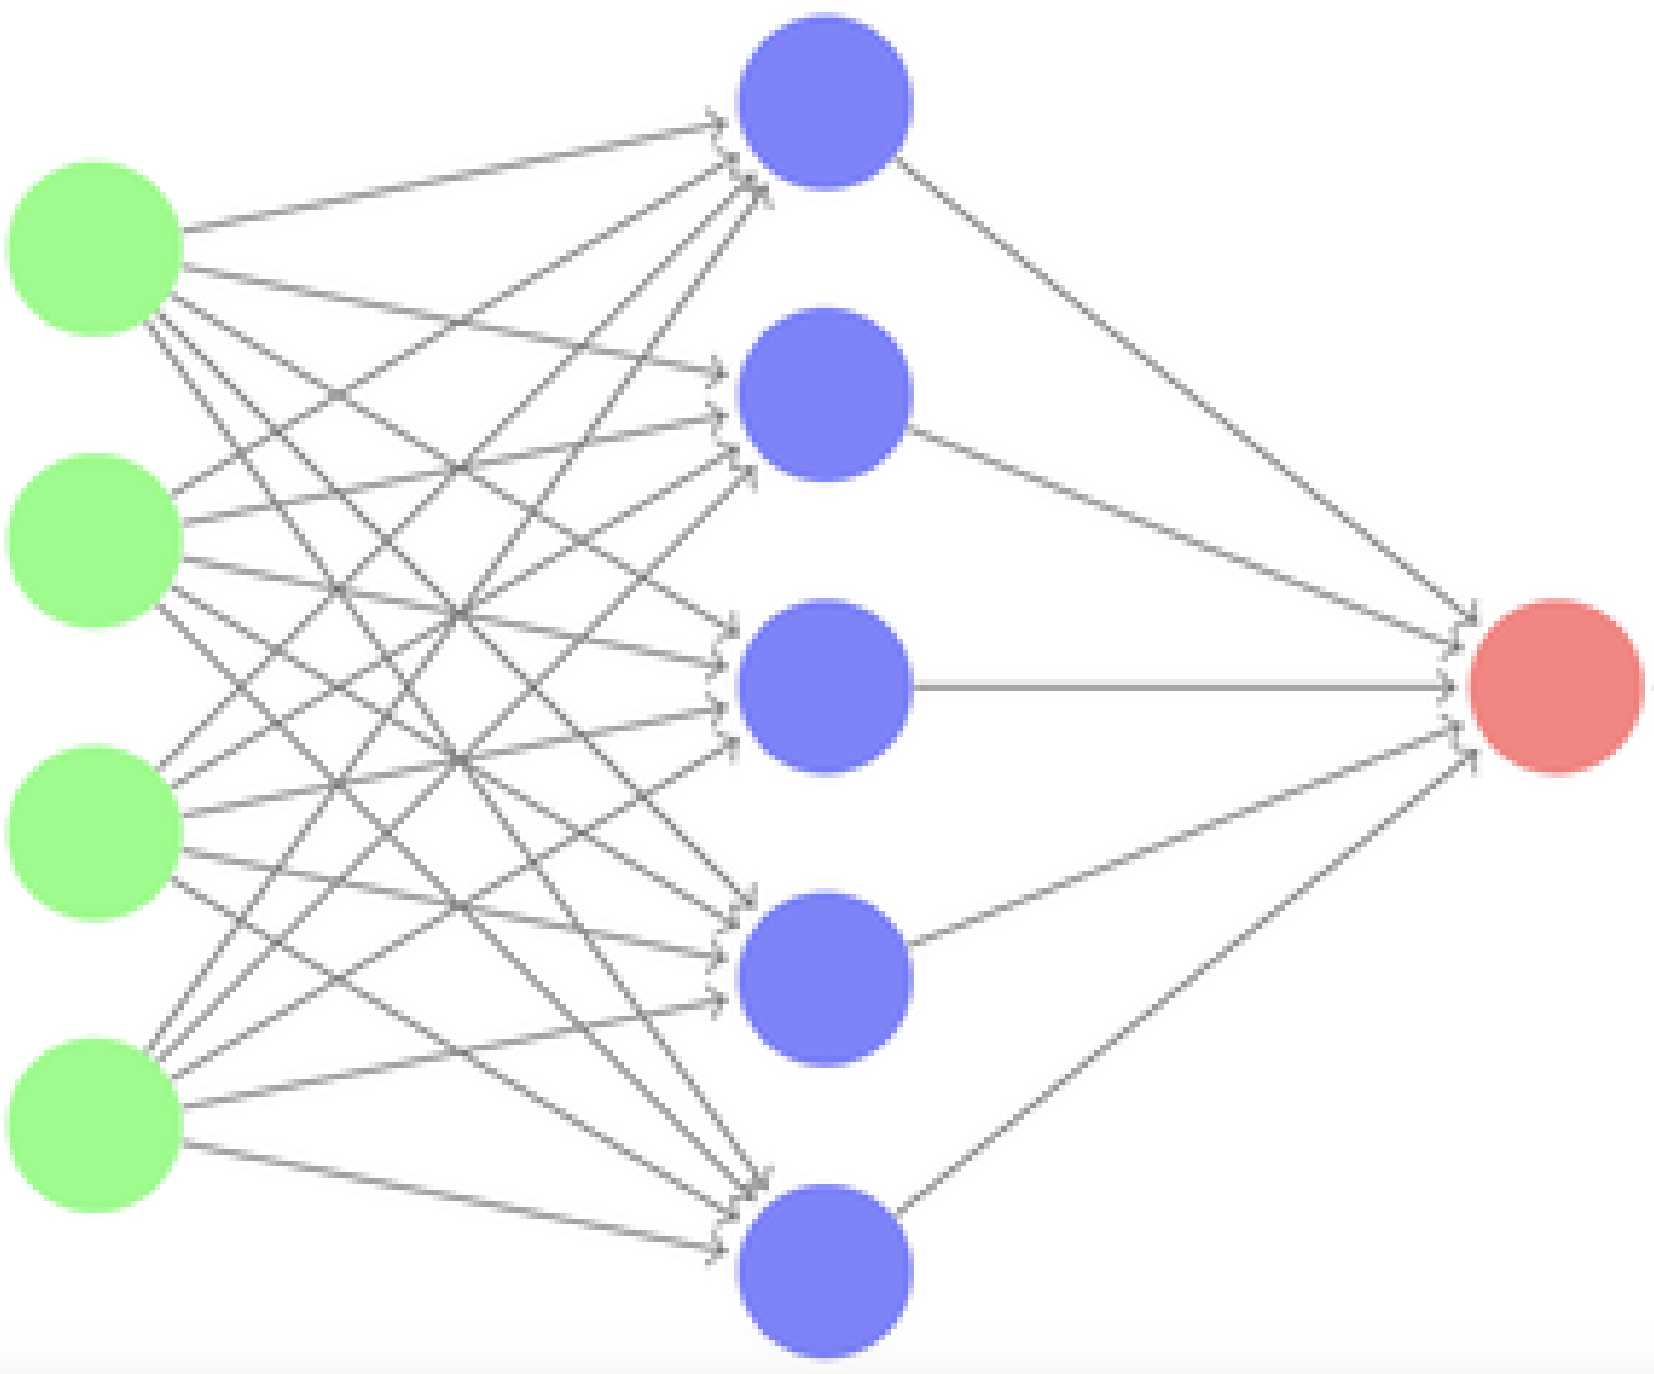
\includegraphics[width=2in]{7/neural-network.png}
\end{center}

In the literature, the circles are called ``neurons,'' matrices are ``fully connected,'' each column is a ``layer'' with implied squashing, each line is a parameter. The goal of these networks is to find $\mu$.

``Personally, I find this part---the `it's like a brain!'---pretty silly. It's just linear algebra separated by nonlinear transformations.'' - S. Rush

\subsubsection{Application Architectures for Neural Networks}

In a typical neural network, we have $x\to\text{Layer 1}\to\text{Layer 2}\to\cdots\to\text{Output}$, where each arrow is a linear map, and in each layer is a non-linear function. In the class before, we talked about classifying the MNIST data set---for this simple model, we had 8000 parameters(!). ``But that's nothing---just yesterday I was working with a model with 1.2 billion parameters.''

Although some of the power of neural networks comes from this flexibility in parameters, much of the interesting work is done in trying to find better neural network architectures that capture more of the essence of the data with fewer parameters. For example, the modern approaches to digit classification are done by convolutional neural networks, where the architecture captures some of the ``local'' information of images.

\begin{example}
\label{speech2}
  [Speech Recognition]
  Suppose we want to map sounds into classes of saying the digits ``one,'' ``two,'' and so on. Recall that the typical approach is to split speech into chunks and perform Fourier transforms to extract features from each chunk.  The problem here is that individual chunks don't necessarily map to single digits, since there's no guarantee the chunk even corresponds to an entire word in speech!

  Instead, what is typically done in this case is convolution using a \emph{kernel} (equivalently, a single weight vector called $w^{\text{tile}}$) that spans several chunks.  Rather than applying learning on the full $\mathbb{R}^{n \cdot 13}$ data set (where $n$ is the number of chunks), we multiply each $k$-chunk stretch of speech by the kernel to obtain $\approx n - k$ chunks.  Based on our choice of kernel, we can take advantage of sparsity to improve structure in the data set.  This is known as a one-dimensional convolution between the kernel, $w^{\text{tile}}$, and the input $\phi(x)$.

    \begin{figure}[!ht]
    \centering
    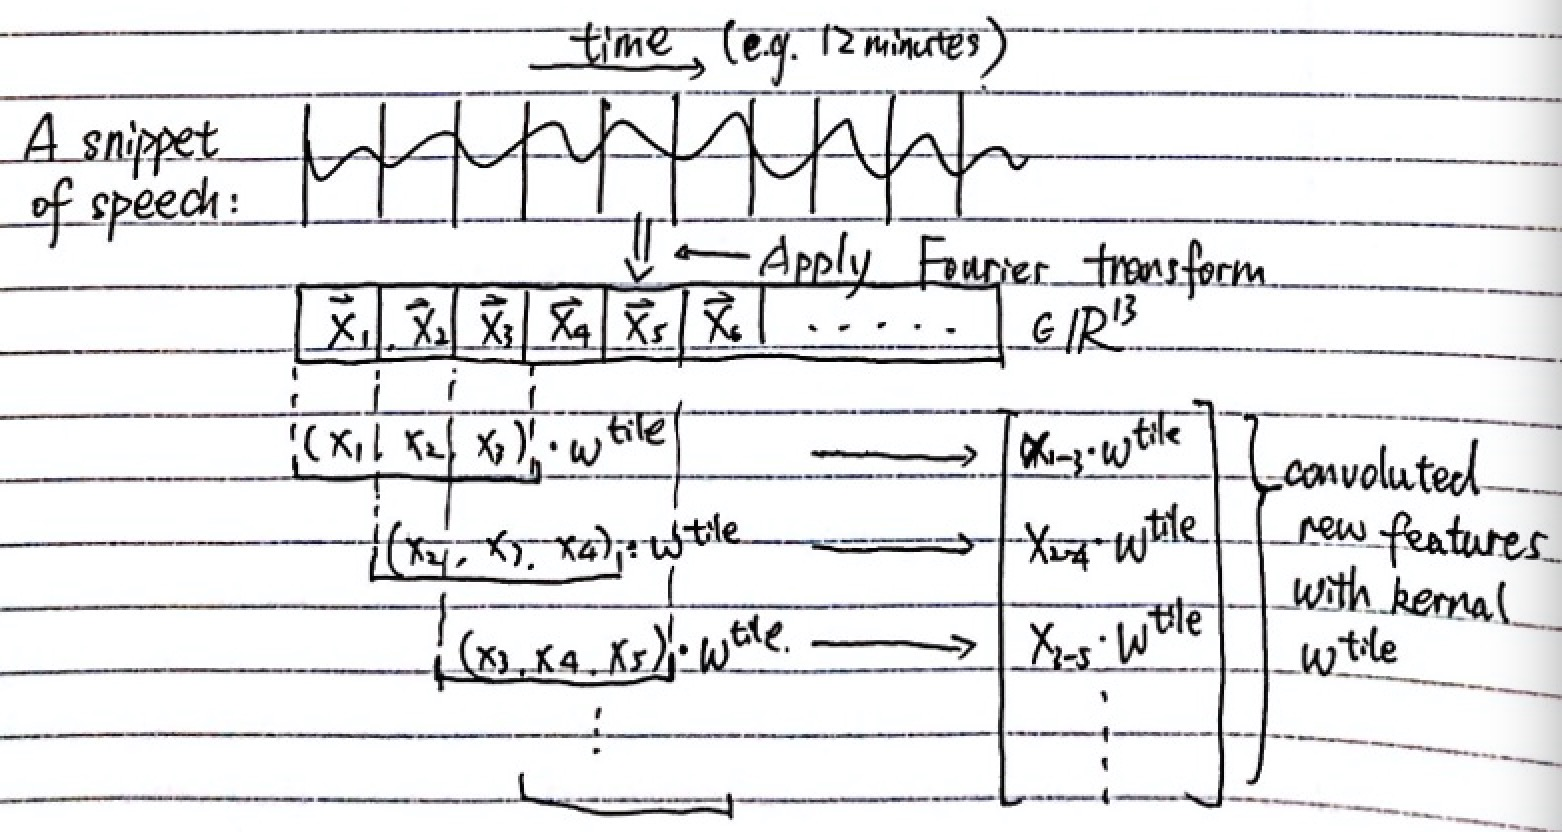
\includegraphics[width = 0.7\textwidth]{speech2.jpg}
    %\vspace{-0.2cm}
    \caption{Convolution architecture in speech recognition in Example~\ref{speech2}}
    %\vspace{-0.4cm}
    \end{figure}
\end{example}

\begin{example}[Image Classification]
  For the case of images, we can do the same as above with two-dimensional convolution, where have blocks in the image instead of tiles. This lets us pick up on information that is very local---e.g., or edges or corners in images, informatoin which can then be recombined in later layers with spectacular success.
\end{example}

\begin{example}[Language Classification]
  Suppose we want to determine whether a movie review was good or bad. Consider the review ``The movie was not very good.'' One way to do this to convert words to vector representations (e.g., via word2vec or glove), since discrete words are difficult to deal with, but vectors let us have a more continuous approach while taking into account the meaning. We can do things like add these vectors up over the course of the review (e.g., a bag-of-words approach). An alternative is to take blocks of words and use a one-dimensional convolution. One advantage of the latter is that it allows you to pick up on structures such as ``not very good,'' which wouldn't be observed in a bag-of-words model, which may pick up on the words ``very'' and ``good'' instead.
\end{example}

\begin{remark}
All of these convolution methods exist in PyTorch under \texttt{nn.conv}.
\end{remark}

\end{document}
